\documentclass[10pt,]{book}
\usepackage{lmodern}
\usepackage{amssymb,amsmath}
\usepackage{ifxetex,ifluatex}
\usepackage{fixltx2e} % provides \textsubscript
\ifnum 0\ifxetex 1\fi\ifluatex 1\fi=0 % if pdftex
  \usepackage[T1]{fontenc}
  \usepackage[utf8]{inputenc}
\else % if luatex or xelatex
  \ifxetex
    \usepackage{mathspec}
  \else
    \usepackage{fontspec}
  \fi
  \defaultfontfeatures{Ligatures=TeX,Scale=MatchLowercase}
\fi
% use upquote if available, for straight quotes in verbatim environments
\IfFileExists{upquote.sty}{\usepackage{upquote}}{}
% use microtype if available
\IfFileExists{microtype.sty}{%
\usepackage{microtype}
\UseMicrotypeSet[protrusion]{basicmath} % disable protrusion for tt fonts
}{}
\usepackage[margin=1in]{geometry}
\usepackage{hyperref}
\PassOptionsToPackage{usenames,dvipsnames}{color} % color is loaded by hyperref
\hypersetup{unicode=true,
            pdftitle={Manual de R},
            colorlinks=true,
            linkcolor=Maroon,
            citecolor=Blue,
            urlcolor=Blue,
            breaklinks=true}
\urlstyle{same}  % don't use monospace font for urls
\usepackage{natbib}
\bibliographystyle{apalike}
\usepackage{color}
\usepackage{fancyvrb}
\newcommand{\VerbBar}{|}
\newcommand{\VERB}{\Verb[commandchars=\\\{\}]}
\DefineVerbatimEnvironment{Highlighting}{Verbatim}{commandchars=\\\{\}}
% Add ',fontsize=\small' for more characters per line
\usepackage{framed}
\definecolor{shadecolor}{RGB}{248,248,248}
\newenvironment{Shaded}{\begin{snugshade}}{\end{snugshade}}
\newcommand{\KeywordTok}[1]{\textcolor[rgb]{0.13,0.29,0.53}{\textbf{{#1}}}}
\newcommand{\DataTypeTok}[1]{\textcolor[rgb]{0.13,0.29,0.53}{{#1}}}
\newcommand{\DecValTok}[1]{\textcolor[rgb]{0.00,0.00,0.81}{{#1}}}
\newcommand{\BaseNTok}[1]{\textcolor[rgb]{0.00,0.00,0.81}{{#1}}}
\newcommand{\FloatTok}[1]{\textcolor[rgb]{0.00,0.00,0.81}{{#1}}}
\newcommand{\ConstantTok}[1]{\textcolor[rgb]{0.00,0.00,0.00}{{#1}}}
\newcommand{\CharTok}[1]{\textcolor[rgb]{0.31,0.60,0.02}{{#1}}}
\newcommand{\SpecialCharTok}[1]{\textcolor[rgb]{0.00,0.00,0.00}{{#1}}}
\newcommand{\StringTok}[1]{\textcolor[rgb]{0.31,0.60,0.02}{{#1}}}
\newcommand{\VerbatimStringTok}[1]{\textcolor[rgb]{0.31,0.60,0.02}{{#1}}}
\newcommand{\SpecialStringTok}[1]{\textcolor[rgb]{0.31,0.60,0.02}{{#1}}}
\newcommand{\ImportTok}[1]{{#1}}
\newcommand{\CommentTok}[1]{\textcolor[rgb]{0.56,0.35,0.01}{\textit{{#1}}}}
\newcommand{\DocumentationTok}[1]{\textcolor[rgb]{0.56,0.35,0.01}{\textbf{\textit{{#1}}}}}
\newcommand{\AnnotationTok}[1]{\textcolor[rgb]{0.56,0.35,0.01}{\textbf{\textit{{#1}}}}}
\newcommand{\CommentVarTok}[1]{\textcolor[rgb]{0.56,0.35,0.01}{\textbf{\textit{{#1}}}}}
\newcommand{\OtherTok}[1]{\textcolor[rgb]{0.56,0.35,0.01}{{#1}}}
\newcommand{\FunctionTok}[1]{\textcolor[rgb]{0.00,0.00,0.00}{{#1}}}
\newcommand{\VariableTok}[1]{\textcolor[rgb]{0.00,0.00,0.00}{{#1}}}
\newcommand{\ControlFlowTok}[1]{\textcolor[rgb]{0.13,0.29,0.53}{\textbf{{#1}}}}
\newcommand{\OperatorTok}[1]{\textcolor[rgb]{0.81,0.36,0.00}{\textbf{{#1}}}}
\newcommand{\BuiltInTok}[1]{{#1}}
\newcommand{\ExtensionTok}[1]{{#1}}
\newcommand{\PreprocessorTok}[1]{\textcolor[rgb]{0.56,0.35,0.01}{\textit{{#1}}}}
\newcommand{\AttributeTok}[1]{\textcolor[rgb]{0.77,0.63,0.00}{{#1}}}
\newcommand{\RegionMarkerTok}[1]{{#1}}
\newcommand{\InformationTok}[1]{\textcolor[rgb]{0.56,0.35,0.01}{\textbf{\textit{{#1}}}}}
\newcommand{\WarningTok}[1]{\textcolor[rgb]{0.56,0.35,0.01}{\textbf{\textit{{#1}}}}}
\newcommand{\AlertTok}[1]{\textcolor[rgb]{0.94,0.16,0.16}{{#1}}}
\newcommand{\ErrorTok}[1]{\textcolor[rgb]{0.64,0.00,0.00}{\textbf{{#1}}}}
\newcommand{\NormalTok}[1]{{#1}}
\usepackage{longtable,booktabs}
\usepackage{graphicx,grffile}
\makeatletter
\def\maxwidth{\ifdim\Gin@nat@width>\linewidth\linewidth\else\Gin@nat@width\fi}
\def\maxheight{\ifdim\Gin@nat@height>\textheight\textheight\else\Gin@nat@height\fi}
\makeatother
% Scale images if necessary, so that they will not overflow the page
% margins by default, and it is still possible to overwrite the defaults
% using explicit options in \includegraphics[width, height, ...]{}
\setkeys{Gin}{width=\maxwidth,height=\maxheight,keepaspectratio}
\IfFileExists{parskip.sty}{%
\usepackage{parskip}
}{% else
\setlength{\parindent}{0pt}
\setlength{\parskip}{6pt plus 2pt minus 1pt}
}
\setlength{\emergencystretch}{3em}  % prevent overfull lines
\providecommand{\tightlist}{%
  \setlength{\itemsep}{0pt}\setlength{\parskip}{0pt}}
\setcounter{secnumdepth}{5}
% Redefines (sub)paragraphs to behave more like sections
\ifx\paragraph\undefined\else
\let\oldparagraph\paragraph
\renewcommand{\paragraph}[1]{\oldparagraph{#1}\mbox{}}
\fi
\ifx\subparagraph\undefined\else
\let\oldsubparagraph\subparagraph
\renewcommand{\subparagraph}[1]{\oldsubparagraph{#1}\mbox{}}
\fi

%%% Use protect on footnotes to avoid problems with footnotes in titles
\let\rmarkdownfootnote\footnote%
\def\footnote{\protect\rmarkdownfootnote}

%%% Change title format to be more compact
\usepackage{titling}

% Create subtitle command for use in maketitle
\newcommand{\subtitle}[1]{
  \posttitle{
    \begin{center}\large#1\end{center}
    }
}

\setlength{\droptitle}{-2em}
  \title{Manual de R}
  \pretitle{\vspace{\droptitle}\centering\huge}
  \posttitle{\par}
  \author{Freddy Hernández Barajas\\
Olga Cecilia Usuga Manco}
  \preauthor{\centering\large\emph}
  \postauthor{\par}
  \predate{\centering\large\emph}
  \postdate{\par}
  \date{2016-12-03}

\usepackage{booktabs}
\usepackage[spanish]{babel}
\decimalpoint
\selectlanguage{spanish}

% Comandos para escribir nombres de paquetes, programas y codigos
\newcommand{\pkg}[1]{{\normalfont\fontseries{b}\selectfont #1}}
\let\proglang=\textsf
\let\code=\texttt

% Para crear el indice
\usepackage{makeidx}
\makeindex

\begin{document}
\maketitle

{
\hypersetup{linkcolor=black}
\setcounter{tocdepth}{1}
\tableofcontents
}
\listoftables
\listoffigures
\chapter*{Prefacio}\label{prefacio}
\addcontentsline{toc}{chapter}{Prefacio}

En este manual de \proglang{R} se explican de forma sencilla las
funciones y procedimientos básicos para un análisis estadístico. Como
complemento a este libro se recomienda consultar \citet{correa2016} para
la construcción de gráficos en \proglang{R}.

\chapter{Medidas de tendencia
central}\label{medidas-de-tendencia-central}

En este capítulo se mostrará cómo obtener las diferentes medidas de
tendencia central con \proglang{R}.

Para ilustrar el uso de las funciones se utilizará una base de datos
llamada \textbf{medidas del cuerpo}, esta base de datos cuenta con 6
variables registradas a un grupo de 36 estudiantes de la universidad.
Las variables son:

\begin{enumerate}
\def\labelenumi{\arabic{enumi}.}
\tightlist
\item
  \texttt{edad} del estudiante (años),
\item
  \texttt{peso} del estudiante (kilogramos),
\item
  \texttt{altura} del estudiante (centímetros),
\item
  \texttt{sexo} del estudiante (Hombre, Mujer),
\item
  \texttt{muneca}: perímetro de la muñeca derecha (centímetros),
\item
  \texttt{biceps}: perímetro del biceps derecho (centímetros).
\end{enumerate}

A continuación se presenta el código para definir la url donde están los
datos, para cargar la base de datos en R y para mostrar por pantalla un
encabezado (usando \texttt{head}) de la base de datos.

\begin{Shaded}
\begin{Highlighting}[]
\NormalTok{url <-}\StringTok{ 'https://raw.githubusercontent.com/fhernanb/datos/master/medidas_cuerpo'}
\NormalTok{datos <-}\StringTok{ }\KeywordTok{read.table}\NormalTok{(}\DataTypeTok{file=}\NormalTok{url, }\DataTypeTok{header=}\NormalTok{T)}
\KeywordTok{head}\NormalTok{(datos)  }\CommentTok{# Para ver el encabezado de la base de datos}
\end{Highlighting}
\end{Shaded}

\begin{verbatim}
##   edad peso altura   sexo muneca biceps
## 1   43 87.3  188.0 Hombre   12.2   35.8
## 2   65 80.0  174.0 Hombre   12.0   35.0
## 3   45 82.3  176.5 Hombre   11.2   38.5
## 4   37 73.6  180.3 Hombre   11.2   32.2
## 5   55 74.1  167.6 Hombre   11.8   32.9
## 6   33 85.9  188.0 Hombre   12.4   38.5
\end{verbatim}

\section{\texorpdfstring{Media \index{media}
\index{mean}}{Media  }}\label{media}

Para calcular la media de una variable cuantitativa se usa la función
\texttt{mean}. Los argumentos básicos de la función \texttt{mean} son
dos y se muestran a continuación.

\begin{Shaded}
\begin{Highlighting}[]
\KeywordTok{mean}\NormalTok{(x, na.rm)}
\end{Highlighting}
\end{Shaded}

\subsection*{Ejemplo}\label{ejemplo}
\addcontentsline{toc}{subsection}{Ejemplo}

Suponga que queremos obtener la altura media del grupo de estudiantes.

Para encontrar la media general se usa la función \texttt{mean} sobre el
vector númerico \texttt{datos\$altura}.

\begin{Shaded}
\begin{Highlighting}[]
\KeywordTok{mean}\NormalTok{(}\DataTypeTok{x=}\NormalTok{datos$altura)}
\end{Highlighting}
\end{Shaded}

\begin{verbatim}
## [1] 171.5556
\end{verbatim}

Del anterior resultado podemos decir que la estatura media o promedio de
los estudiantes es 171.5555556 centímetros.

\subsection*{Ejemplo}\label{ejemplo-1}
\addcontentsline{toc}{subsection}{Ejemplo}

Suponga que ahora queremos la altura media pero diferenciando por sexo.

Para hacer esto se debe primero dividir o partir el vector de altura
según los niveles de la variable sexo, esto se consigue por medio de la
función \texttt{split} y el resultado será una lista con tantos
elementos como niveles tenga la variable sexo. Luego a cada uno de los
elementos de la lista se le aplica la función \texttt{mean} con la ayuda
de \texttt{sapply} o \texttt{tapply}. A continuación el código completo
para obtener las alturas medias para hombres y mujeres.

\begin{Shaded}
\begin{Highlighting}[]
\KeywordTok{sapply}\NormalTok{(}\KeywordTok{split}\NormalTok{(}\DataTypeTok{x=}\NormalTok{datos$altura, }\DataTypeTok{f=}\NormalTok{datos$sexo), mean)}
\end{Highlighting}
\end{Shaded}

\begin{verbatim}
##   Hombre    Mujer 
## 179.0778 164.0333
\end{verbatim}

El resultado es un vector con dos elementos, vemos que la altura media
para hombres es 179.0777778 centímetros y que para las mujeres es de
164.0333333 centímetros.

¿Qué sucede si se usa \texttt{tapply} en lugar de \texttt{sapply}?
Substituya en el código anterior la función \texttt{sapply} por
\texttt{tapply} y observe la diferencia entre los resultados.

\subsection*{Ejemplo}\label{ejemplo-2}
\addcontentsline{toc}{subsection}{Ejemplo}

Suponga que se tiene el vector \texttt{edad} con las edades de siete
personas y supóngase que para el individuo cinco no se tiene información
de su edad, eso significa que el vector tendrá un \texttt{NA} en la
quinta posición.

¿Cuál será la edad promedio del grupo de personas?

\begin{Shaded}
\begin{Highlighting}[]
\NormalTok{edad <-}\StringTok{ }\KeywordTok{c}\NormalTok{(}\DecValTok{18}\NormalTok{, }\DecValTok{23}\NormalTok{, }\DecValTok{26}\NormalTok{, }\DecValTok{32}\NormalTok{, }\OtherTok{NA}\NormalTok{, }\DecValTok{32}\NormalTok{, }\DecValTok{29}\NormalTok{)}
\KeywordTok{mean}\NormalTok{(}\DataTypeTok{x=}\NormalTok{edad)}
\end{Highlighting}
\end{Shaded}

\begin{verbatim}
## [1] NA
\end{verbatim}

Al correr el código anterior se obtiene un error y es debido al símbolo
\texttt{NA} en la quinta posición. Para calcular la media sólo con los
datos de los cuales se tiene información, se incluye el argumento
\texttt{na.rm\ =\ TRUE} para que R remueva los \texttt{NA}. El código
correcto a usar en este caso es:

\begin{Shaded}
\begin{Highlighting}[]
\KeywordTok{mean}\NormalTok{(}\DataTypeTok{x=}\NormalTok{edad, }\DataTypeTok{na.rm=}\OtherTok{TRUE}\NormalTok{)}
\end{Highlighting}
\end{Shaded}

\begin{verbatim}
## [1] 26.66667
\end{verbatim}

De este último resultado se obtiene que la edad promedio de los
individuos es 26.67 años.

\section{\texorpdfstring{Mediana \index{mediana}
\index{median}}{Mediana  }}\label{mediana}

Para calcular la mediana de una variable cantitativa se usa la función
\texttt{median}. Los argumentos básicos de la función \texttt{median}
son dos y se muestran a continuación.

\begin{Shaded}
\begin{Highlighting}[]
\KeywordTok{median}\NormalTok{(x, na.rm)}
\end{Highlighting}
\end{Shaded}

\subsection*{Ejemplo}\label{ejemplo-3}
\addcontentsline{toc}{subsection}{Ejemplo}

Calcular la edad mediana para los estudiantes de la base de datos.

Para obtener la mediana usamos el siguiente código:

\begin{Shaded}
\begin{Highlighting}[]
\KeywordTok{median}\NormalTok{(}\DataTypeTok{x=}\NormalTok{datos$edad)}
\end{Highlighting}
\end{Shaded}

\begin{verbatim}
## [1] 28
\end{verbatim}

y obtenemos que la mitad de los estudiantes tienen edades mayores o
iguales a 28 años.

El resultado anterior se pudo haber obtenido con la función
\texttt{quantile} e indicando que se desea el cuantil 50 así:

\begin{Shaded}
\begin{Highlighting}[]
\KeywordTok{quantile}\NormalTok{(}\DataTypeTok{x=}\NormalTok{datos$edad, }\DataTypeTok{probs=}\FloatTok{0.5}\NormalTok{)}
\end{Highlighting}
\end{Shaded}

\begin{verbatim}
## 50% 
##  28
\end{verbatim}

\section{\texorpdfstring{Moda \index{moda}}{Moda }}\label{moda}

La moda de una variable cuantitativa corresponde a valor o valores que
más se repiten, una forma sencilla de encontrar la moda es construir una
tabla de frecuencias y observar los valores con mayor frecuencia.

\subsection*{Ejemplo}\label{ejemplo-4}
\addcontentsline{toc}{subsection}{Ejemplo}

Calcular la moda para la variable edad de la base de datos de
estudiantes.

Se construye la tabla con la función \texttt{table} y se crea el objeto
\texttt{tabla} para almacenarla.

\begin{Shaded}
\begin{Highlighting}[]
\NormalTok{tabla <-}\StringTok{ }\KeywordTok{table}\NormalTok{(datos$edad)}
\NormalTok{tabla}
\end{Highlighting}
\end{Shaded}

\begin{verbatim}
## 
## 19 20 21 22 23 24 25 26 28 29 30 32 33 35 37 40 43 45 51 55 65 
##  1  1  1  3  2  1  5  3  2  1  2  1  1  2  3  1  2  1  1  1  1
\end{verbatim}

Al mirar con detalle la tabla anterior se observa que el valor que más
se repite es la edad de 25 años en 5 ocasiones. Si la tabla hubiese sido
mayor, la inspección visual nos podría tomar unos segundos o hasta
minutos y podríamos equivocarnos, por esa razón es mejor ordenar los
resultados de la tabla.

Para observar los valores con mayor frecuencia de la tabla se puede
ordenar la tabla usando la función \texttt{sort} de la siguiente manera:

\begin{Shaded}
\begin{Highlighting}[]
\KeywordTok{sort}\NormalTok{(tabla, }\DataTypeTok{decreasing=}\OtherTok{TRUE}\NormalTok{)}
\end{Highlighting}
\end{Shaded}

\begin{verbatim}
## 
## 25 22 26 37 23 28 30 35 43 19 20 21 24 29 32 33 40 45 51 55 65 
##  5  3  3  3  2  2  2  2  2  1  1  1  1  1  1  1  1  1  1  1  1
\end{verbatim}

De esta manera se ve fácilmente que la variable edad es unimodal con
valor de 25 años.

\chapter{Medidas de variabilidad}\label{medidas-de-variabilidad}

En este capítulo se mostrará cómo obtener las diferentes medidas de
variabilidad con \proglang{R}.

Para ilustrar el uso de las funciones se utilizará la base de datos
llamada \textbf{aptos2015}, esta base de datos cuenta con 11 variables
registradas a apartamentos usados en la ciudad de Medellín. Las
variables son:

\begin{enumerate}
\def\labelenumi{\arabic{enumi}.}
\tightlist
\item
  \texttt{precio}: precio de venta del apartamento (millones de pesos),
\item
  \texttt{mt2}: área del apartamento (\(m^2\)),
\item
  \texttt{ubicación}: lugar de ubicación del aparamentos en la ciudad
  (cualitativa),
\item
  \texttt{estrato}: nivel socioeconómico donde está el apartamento (2 a
  6),
\item
  \texttt{alcobas}: número de alcobas del apartamento,
\item
  \texttt{banos}: número de baños del apartamento,
\item
  \texttt{balcon}: si el apartamento tiene balcón (si o no),
\item
  \texttt{parqueadero}: si el apartamento tiene parqueadero (si o no),
\item
  \texttt{administracion}: valor mensual del servicio de administración
  (millones de pesos),
\item
  \texttt{avaluo}: valor del apartamento en escrituras (millones de
  pesos),
\item
  \texttt{terminado}: si el apartamento se encuentra terminado (si o
  no).
\end{enumerate}

A continuación se presenta el código para definir la url donde están los
datos, para cargar la base de datos en R y para mostrar por pantalla un
encabezado (usando \texttt{head}) de la base de datos.

\begin{Shaded}
\begin{Highlighting}[]
\NormalTok{url <-}\StringTok{ 'https://raw.githubusercontent.com/fhernanb/datos/master/aptos2015'}
\NormalTok{datos <-}\StringTok{ }\KeywordTok{read.table}\NormalTok{(}\DataTypeTok{file=}\NormalTok{url, }\DataTypeTok{header=}\NormalTok{T)}
\KeywordTok{head}\NormalTok{(datos)  }\CommentTok{# Para ver el encabezado de la base de datos}
\end{Highlighting}
\end{Shaded}

\begin{verbatim}
##   precio   mt2 ubicacion estrato alcobas banos balcon parqueadero
## 1     79 43.16     norte       3       3     1     si          si
## 2     93 56.92     norte       2       2     1     si          si
## 3    100 66.40     norte       3       2     2     no          no
## 4    123 61.85     norte       2       3     2     si          si
## 5    135 89.80     norte       4       3     2     si          no
## 6    140 71.00     norte       3       3     2     no          si
##   administracion   avaluo terminado
## 1          0.050 14.92300        no
## 2          0.069 27.00000        si
## 3          0.000 15.73843        no
## 4          0.130 27.00000        no
## 5          0.000 39.56700        si
## 6          0.120 31.14551        si
\end{verbatim}

\section{\texorpdfstring{Rango \index{rango}
\index{range}}{Rango  }}\label{rango}

Para calcular el rango de una variable cuantitativa se usa la función
\texttt{range}. Los argumentos básicos de la función \texttt{range} son
dos y se muestran abajo.

\begin{Shaded}
\begin{Highlighting}[]
\KeywordTok{range}\NormalTok{(x, na.rm)}
\end{Highlighting}
\end{Shaded}

La función \texttt{range} entrega el valor mínimo y máximo de la
variable ingresada y el valor de rango (\(max - min\)) se puede obtener
restando del máximo el mínimo.

\subsection*{Ejemplo}\label{ejemplo-5}
\addcontentsline{toc}{subsection}{Ejemplo}

Suponga que queremos obtener el rango para la variable precio de los
apartamentos.

Para obtener el rango usamos el siguiente código.

\begin{Shaded}
\begin{Highlighting}[]
\KeywordTok{range}\NormalTok{(datos$precio)}
\end{Highlighting}
\end{Shaded}

\begin{verbatim}
## [1]   25 1700
\end{verbatim}

\begin{Shaded}
\begin{Highlighting}[]
\KeywordTok{max}\NormalTok{(datos$precio) -}\StringTok{ }\KeywordTok{min}\NormalTok{(datos$precio)}
\end{Highlighting}
\end{Shaded}

\begin{verbatim}
## [1] 1675
\end{verbatim}

Del resultado anterior podemos ver que los precios de todos los
apartamentos van desde 25 hasta 1700 millones de pesos, es decir, el
rango de la variables precio es 1675 millones de pesos.

\subsection*{Ejemplo}\label{ejemplo-6}
\addcontentsline{toc}{subsection}{Ejemplo}

Suponga que queremos obtener nuevamente el rango para la variable precio
de los apartamentos pero diferenciando por el estrato.

Primero vamos a crear una función auxiliar llamada \texttt{myrange} que
calculará el rango directamente (\(max - min\)). Luego vamos a partir la
información de los precios por cada estrato usando \texttt{split}, la
partición se almacenará en la lista \texttt{precios}. Finalmente se
aplicará la función \texttt{myrange} a la lista \texttt{precios} para
obtener los rangos del precio por estrato socioeconómico. El código para
realizar esto se muestra a continuación.

\begin{Shaded}
\begin{Highlighting}[]
\NormalTok{myrange <-}\StringTok{ }\NormalTok{function(x) }\KeywordTok{max}\NormalTok{(x) -}\StringTok{ }\KeywordTok{min}\NormalTok{(x)}
\NormalTok{precios <-}\StringTok{ }\KeywordTok{split}\NormalTok{(datos$precio, }\DataTypeTok{f=}\NormalTok{datos$estrato)}
\KeywordTok{sapply}\NormalTok{(precios, myrange)}
\end{Highlighting}
\end{Shaded}

\begin{verbatim}
##    2    3    4    5    6 
##  103  225  610 1325 1560
\end{verbatim}

De los resultados podemos ver claramente que a medida que aumenta de
estrato el rango (variabilidad) del precio de los apartamentos aumenta.
Apartamentos de estrato bajo tienden a tener precios similares mientras
que los precios de venta para apartamentos de estratos altos tienden a
ser muy diferentes entre si.

\chapter{Medidas de posición}\label{medidas-de-posicion}

En este capítulo se mostrará cómo obtener las diferentes medidas de

\chapter{Medidas de correlación}\label{medidas-de-correlacion}

En este capítulo se mostrará cómo obtener las diferentes medidas de

\chapter{Funciones básicas de R}\label{funciones-basicas-de-r}

En este capítulo se

\chapter{Creación de funciones en R}\label{creacion-de-funciones-en-r}

En este capítulo se

\chapter{Distribuciones discretas}\label{distribuciones-discretas}

En este capítulo se

\chapter{Distribuciones continuas}\label{distribuciones-continuas}

En este capítulo se

\chapter{Distribuciones continuas}\label{distribuciones-continuas-1}

En este capítulo se

\chapter{Aproximación de integrales}\label{aproximacion-de-integrales}

En este capítulo se mostrará cómo aproximar integrales en una y varias
dimensiones.

\section{Aproximación de Laplace
unidimensional}\label{aproximacion-de-laplace-unidimensional}

Esta aproximación es útil para obtener el valor de una integral usando
la expansión de Taylor para una función \(f(x)\) unimodal en \(\Re\), en
otras palabras lo que interesa es:
\[ I = \int_{-\infty}^{\infty} f(x) d(x)\] Al hacer una expansión de
Taylor de segundo orden para \(\log(f(x))\) en su moda \(x_0\) el
resultado es:
\[ \log(f(x)) \approx \log(f(x_0)) + \frac{\log(f)^\prime(x_0)}{1!} (x-x_0) + \frac{\log(f)^{\prime \prime}(x_0)}{2!} (x-x_0)^2 \]
El segundo término de la suma se anula porque \(\log(f)^\prime(x_0)=0\)
por ser \(x_0\) el valor donde está el máximo de \(\log(f(x))\). La
expresión anterior se simplifica en:
\[ \log(f(x)) \approx \log(f(x_0)) + \frac{\log(f)^{\prime \prime}(x_0)}{2!} (x-x_0)^2 \]
al aislar \(f(x)\) se tiene que

\begin{equation} \label{fx}
f(x) \approx f(x_0)  \exp \left( -\frac{c}{2} (x-x_0)^2 \right)
\end{equation}

donde \(c=-\frac{d^2}{dx^2} \log(f(x)) \bigg|_{x=x_0}\).

La expresión \ref{fx} se puede reescribir de manera que aparezca el
núcleo de la función de densidad de la distribución normal con media
\(x_0\) y varianza \(1/c\), a continuación la expresión

\[
f(x) \approx f(x_0) \frac{\sqrt{2 \pi / c}}{\sqrt{2 \pi / c}}  \exp \left( -\frac{1}{2} \left( \frac{x-x_0}{1/\sqrt{c}} \right)^2 \right)
\] Así al calcular la integral de \(f(x)\) en \(\Re\) se tiene que:

\begin{equation} \label{aprox_laplace}
I = \int_{-\infty}^{\infty} f(x) d(x) = f(x_0) \sqrt{2 \pi / c}
\end{equation}

\subsection{Ejemplo}\label{ejemplo-7}

Calcular la integral de \(f(x)=\exp \left( -(x-1.5)^2 \right)\) en
\(\Re\) utilizando la aproximación de Laplace.

Primero vamos a dibujar la función \(f(x)\) para ver en dónde está su
moda \(x_0\).

\begin{Shaded}
\begin{Highlighting}[]
\NormalTok{fun <-}\StringTok{ }\NormalTok{function(x) }\KeywordTok{exp}\NormalTok{(-(x}\FloatTok{-1.5}\NormalTok{)^}\DecValTok{2}\NormalTok{)}
\KeywordTok{curve}\NormalTok{(fun, }\DataTypeTok{from=}\NormalTok{-}\DecValTok{5}\NormalTok{, }\DataTypeTok{to=}\DecValTok{5}\NormalTok{, }\DataTypeTok{ylab=}\StringTok{'f(x)'}\NormalTok{, }\DataTypeTok{las=}\DecValTok{1}\NormalTok{)}
\end{Highlighting}
\end{Shaded}

\begin{figure}[htbp]
\centering
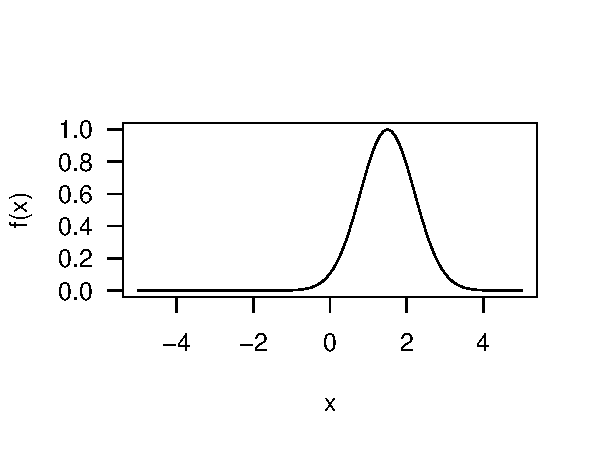
\includegraphics{11_Aprox_Int_files/figure-latex/unnamed-chunk-1-1.pdf}
\caption{\label{fig:unnamed-chunk-1}Perfil de la función f(x).}
\end{figure}

Visualmente se nota que la moda está cerca del valor 1.5 y para
determinar numéricamente el valor de la moda \(x_0\) se usa la función
\texttt{optimize}, los resultados se almacenan en el objeto
\texttt{res}. El valor de la moda corresponde al elemento
\texttt{maximum} del objeto \texttt{res}.

\begin{Shaded}
\begin{Highlighting}[]
\NormalTok{res <-}\StringTok{ }\KeywordTok{optimize}\NormalTok{(fun, }\DataTypeTok{interval=}\KeywordTok{c}\NormalTok{(-}\DecValTok{10}\NormalTok{, }\DecValTok{10}\NormalTok{), }\DataTypeTok{maximum=}\OtherTok{TRUE}\NormalTok{)}
\NormalTok{res}
\end{Highlighting}
\end{Shaded}

\begin{verbatim}
## $maximum
## [1] 1.499997
## 
## $objective
## [1] 1
\end{verbatim}

Para determinar el valor de \(c\) de la expresión \ref{aprox_laplace} se
utiliza el siguiente código.

\begin{Shaded}
\begin{Highlighting}[]
\KeywordTok{require}\NormalTok{(}\StringTok{"numDeriv"}\NormalTok{)}
\NormalTok{constant <-}\StringTok{ }\NormalTok{-}\StringTok{ }\KeywordTok{as.numeric}\NormalTok{(}\KeywordTok{hessian}\NormalTok{(fun, res$maximum))}
\end{Highlighting}
\end{Shaded}

Para obtener la aproximación de la integral se usa la expresión
\ref{aprox_laplace} y para tener un punto de comparación se evalua la
integral usando la función \texttt{integrate}, a continuación el código.

\begin{Shaded}
\begin{Highlighting}[]
\KeywordTok{fun}\NormalTok{(res$maximum) *}\StringTok{ }\KeywordTok{sqrt}\NormalTok{(}\DecValTok{2}\NormalTok{*pi/constant)}
\end{Highlighting}
\end{Shaded}

\begin{verbatim}
## [1] 1.772454
\end{verbatim}

\begin{Shaded}
\begin{Highlighting}[]
\KeywordTok{integrate}\NormalTok{(fun, -}\OtherTok{Inf}\NormalTok{, }\OtherTok{Inf}\NormalTok{)  }\CommentTok{# Para comparar}
\end{Highlighting}
\end{Shaded}

\begin{verbatim}
## 1.772454 with absolute error < 1.5e-06
\end{verbatim}

De los anteriores resultados vemos que la aproximación es buena.

\bibliography{packages,book}

\printindex


\end{document}
